\section{Implementation}

This section discusses the implementation of the Carat developer API prototype. The API aims to provide mobile application developers the ability to discover how a client mobile device's system settings and state affect the energy consumption of the device.

The design of such a service poses multiple challenges, as discussed in~\cite{7840871}. The dataset itself is large and incrementally changing as time passes, which makes static statistical analysis inconvenient. It is therefore practical to design the service in such a way that the analysis can be executed dynamically whenever the API is accessed. Another challenge is to protect the privacy of the participants of the Carat project.

Association rules were selected as the basis of the API for two reasons. First, the association rules effectively hide all the details about individual Carat users, protecting their privacy, while also enabling reasonably detailed view on how a devices system settings and state affect the energy consumption. Secondly, efficient parallel algorithms exist for generating association rules from huge datasets as discussed in detail in chapter~\ref{association analysis}.

As discussed in~\cite{7840871}, the intention of the Carat API is to allow application developers to retrieve information about their application by authenticating with their developer key. The prototype described here, does not include authentication of application developers, but rather demonstrates the functionality that the API could offer provided that an authentication has been successfully completed. 

\begin{figure}[!htbp]
	\centering
	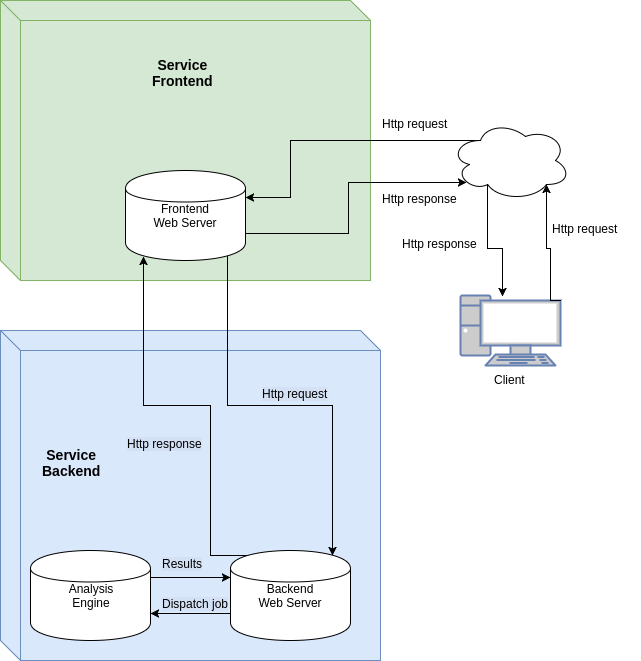
\includegraphics[width=\textwidth]{images/carat-prototype-architecture.png}
	\caption{High level network architecture of the Carat API prototype}
	\label{figure:carat-api-network-prototype}
\end{figure}         

The implementation consists of three main components. These are the front end web server, back end web server and the analysis engine. Figure~\ref{figure:carat-api-network-prototype} shows network level layout of these components and the way these components communicate when the API is accessed. When a client accesses the API, the following flow of requests takes place:
\begin{enumerate}
	\item Client sends a HTTP request to the front end server. The request may contain parameters that control the way the association rules are generated.
	\item Front end web server sends a HTTP request to the back end web server passing along the parameters from the client.
	\item The back end web server dispatches a job to the analysis engine running on SPARK. Parameters provided by the client are used to control the analysis.
	\item Analysis engine sends generated association rules to the back end web server.
	\item Back end server sends HTTP response containing the generated rules to the front end web server.
	\item Front end server uses the association rules to generate a view for the client.  
\end{enumerate}

Figure~\ref{figure:carat-api-network-prototype} shows the flow of control between the different components of the Carat API. The prototype only implements the frontend and the backend of the service. Implementing load balancing and authentication falls outside the scope of this thesis. Some implementation constraints of the authentication module are discussed in~\cite{7840871}.     

\subsection{Service Front End}

\subsection{Service Back End}

\subsection{Analysis Engine}

\begin{wrapfigure}{r}{0.35\textwidth}
	\vspace{-110pt}
	\begin{center}
		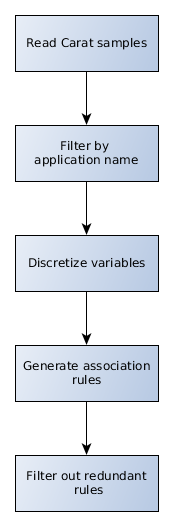
\includegraphics[width=0.3\textwidth]{images/analysis_engine_flow_graph.png}
	\end{center}
	\caption{Overview of the analysis engine pipeline}
	\label{figure:analysis-engine-flow-graph}
\end{wrapfigure}

The primary function of the analysis engine is to generate association rules from the Carat data based on provided query parameters. The query parameters consist of application name, minimum confidence, minimum support and an optional list of attribute names which are to be excluded from the analysis. The application name is used to filter out all Carat energy rate samples in which the the application is not present. The minimum support and minimum confidence parameters affect the association rule generation as described in chapter~\ref{association analysis}. The excluded attributes list controls the association rule generation by completely ignoring all included attributes.    

%\begin{figure}[!htbp]
%	\centering
%	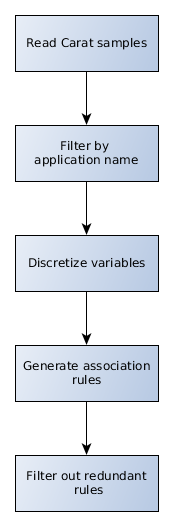
\includegraphics[width=0.25\textwidth]{images/analysis_engine_flow_graph.png}
%	\caption{Overview of the analysis engine pipeline}
%	\label{figure:analysis-engine-flow-graph}
%\end{figure}    
 
Figure~\ref{figure:analysis-engine-flow-graph} describes the process of generating association rules as a simple pipeline consisting of four steps. We will now go through each step providing snippets of code, taken from the analysis engine implementation, that will shed light on the implementation in Spark programming framework. 

Reading Carat samples is very simple in Spark, as is evident from the following code snippet.  

\begin{minipage}{\linewidth}
\begin{lstlisting}[language=scala]
def readCaratRates(sampleDir: String)(implicit sc: SparkContext): RDD[fi.helsinki.cs.nodes.carat.sample.Rate] = {
	sc.objectFile[fi.helsinki.cs.nodes.carat.sample.Rate](s"${sampleDir}")
}
\end{lstlisting}
\end{minipage}

The $objectFile$ method of the $SparkContext$ object will read the dataset from a given directory. The dataset is stored as an RDD (Resilient Distributed Dataset), that is serialized to the disk in a folder given by the $sampleDir$ parameter. RDD is is the data structure that Spark framework uses to store, access and transform distributed datasets. The Carat samples are initially read as instances of class $fi.helsinki.cs.nodes.carat.sample.Rate$. Each $Rate$ object contains two consecutive samples from a mobile device. From these samples, the system settings and running mobile applications can be extracted as described in chapter~\ref{carat data}  

The next task that the analysis engine carry out, is to filter out all Carat rate samples where the requested application was not running. Using the $readCaratRates$ method, one can compose an expression which reads Carat rate data objects, filters out all rate objects that do not have the requested application running and transforms the resulting rate objects to a simplified object type of class $Sample$. 

\begin{minipage}{\linewidth}
\begin{lstlisting}[language=scala]
val samples = readCaratRates(ratePath).collect {
	case rate if rate.allApps().contains(applicationName) => 
		Sample.fromCaratRate(rate)
}
\end{lstlisting}
\end{minipage}  
The $collect$ is a method defined for all instances of class $RDD[T]$ (where $T$ is a type parameter). It is analogous to the $collect$ method from Scala standard library, taking a partial function of signature $PartialFunction[T, U]$  (where $T$ and $U$ are type parameters) and returning a new instance of $RDD[U]$, containing the image of the $RDD[T]$ mapped by the partial function.
        
The $Sample$ is a simple case class that merely stores all the relevant system settings. The case class also has a companion object, in which the method $fromCaratRate$ is defined. The method simply constructs a $Sample$ instance from a $Rate$ instance. 

\begin{minipage}{\linewidth}
\begin{lstlisting}[language=scala]
case class Sample(
	rate: Double,
	cpu: Double,
	distance: Double,
	temp: Double,
	voltage: Double,
	screen: Double,
	mobileNetwork: String,
	network: String,
	wifiStrength: Double,
	wifiSpeed: Double
)
\end{lstlisting}
\end{minipage}  



From usability perspective, generating the association rules should be fast enough not to hinder interactive use, which implies that the rule generation should not take more than a couple of seconds. However, heavily optimizing the analysis engine is outside the scope of this thesis. In practice, the implementation described here achieves run times of a couple of minutes with a rather modest dataset size of 16 gigabytes.


   